%----------------------------------------------------------------------------------------
%	PACKAGES AND DOCUMENT CONFIGURATIONS
%----------------------------------------------------------------------------------------

\documentclass{article}


\usepackage{graphicx} % Required for the inclusion of images
\graphicspath{{figures/}}
\usepackage{subfigure} % Required for the inclusion of images
\usepackage{natbib} % Required to change bibliography style to APA
\usepackage{amsmath} % Required for some math elements 
\usepackage{listings}
\usepackage{xcolor}
\usepackage{fontspec}
\usepackage{ctex}
\usepackage{geometry}
\geometry{a4paper,scale=0.8}
\renewcommand{\contentsname}{\centerline{目录}}
\setmonofont{Consolas}
\lstset{
basicstyle=\ttfamily\footnotesize,%
escapeinside=``,%
keywordstyle=\color{black},%\bfseries, \underbar,%
identifierstyle={},%
tabsize=4,
commentstyle=\color{blue},%
stringstyle=\ttfamily,%
%labelstyle=\tiny,%
extendedchars=false,%
linewidth=\textwidth,%
numbers=left,%
numberstyle=\tiny \color{blue},%
frame=trbl%
}
%点列
%\begin{itemize}
%\item[$\bullet$]Get familiar with Y86 assembly language.
%\end{itemize}

%小标题
%\begin{center}
%{\ttfamily rsum.ys}
%\end{center}
%代码
%\begin{lstlisting}[language={[ANSI]C}]
%\end{lstlisting}
%点列和浮动体图表和ref
%\begin{itemize}
%\item[$\bullet$]{\ttfamily sum.ys} (Figure \ref{Part A: sum.ys})\\
%\end{itemize}
%\begin{figure}[htbp]%figure浮动体环境 [htbp]指定位置
%		\centering%居中排版
%		\includegraphics{A_sum}
%		\caption{Part A  {\ttfamily sum.ys}} \label{Part A: sum.ys}%标题 自动编号 label标签
%\end{figure}


%\usepackage{times} % Uncomment to use the Times New Roman font

%----------------------------------------------------------------------------------------
%	DOCUMENT INFORMATION
%----------------------------------------------------------------------------------------

\title{\textbf{操作系统课程设计Project 4\\Scheduling Algorithms}} % Title

\author{姓名: 郭倩昀  
\\班级: F1903303  
\\学号: 519021910095  
\\Email: guoqianyun@sjtu.edu.cn} % Author name and email
\date{\today} % Date for the report
\begin{document}
\maketitle % Insert the title, author and date
\tableofcontents
\section{Scheduling Algorithms}
\subsection{实验内容与目标}
\begin{itemize}
\item[$\bullet$]利用C语言实现不同的进程调度算法\\
根据本project提供的Makefile文件,结合提供cpu,list,driver,task文件分析,需要我们设计shedule\_rr.c, shedule\_sjf.c, shedule\_fcfs.c, shedule\_priority.c, shedule\_priority\_rr.c一共五个程序分别实现round-robin(RR), shortest-job-first(SJF), first-come,first-served(FCFS), priority scheduling, priority with round-robin五种进程调度算法。
\item[$\bullet$]分配tid时应对竞态条件
\item[$\bullet$]分别为调度算法计算平均周转时间,平均等待时间,平均响应时间。
\end{itemize}
%%%%%%%%%%%%%%%%%%%%%%%%%%%%%%%%%%%%%%%%%%
\subsection{FCFS}
\subsubsection{实验过程及步骤}
\begin{itemize}
\item[$\bullet$]修改task.h文件\\
为支持给调度算法计算平均周转时间,平均等待时间,平均响应时间的功能,修改task.h文件,给结构体task增加辅助计算的记录进程的arrival time,waiting time,last execution time,response time,turnaround time等信息。
\item[$\bullet$]创建全局变量\\
创建任务列表头结点head。另外为支持计算,分别创建全局变量记录当前时间,任务计数,总体等待时间,总体响应时间,总体周转时间和进程tid数值。
\item[$\bullet$]设计add函数\\
根据参数的进程名称,优先级和运行时间创建Task类型的对象并相应赋值,其中任务的tid利用\_\_sync\_fetch\_and\_add函数获得。将Task类中arrival time和last execution time设为当前时间,其他初始化为0。最后将创建好的task插入到任务列表中。
\item[$\bullet$]设计next\_tsk()函数运行下一个进程\\
由于是FCFS调度,根据任务列表插入方式,最先插入的进程在任务列表的最后,每次查找任务列表的最后一个并执行,然后将任务从任务列表中移除,并更新当前时间。另外需要为该进程计算相应的周转时间,等待时间,响应时间并更新全局变量记录信息。
\item[$\bullet$]设计调度函数schedule()\\
当任务列表不为空的时候,就调用next\_tsk()函数运行下一个进程。当任务列表全部完成,打印计算结果。
\end{itemize}
\subsubsection{实验代码}
\begin{center}
{\ttfamily task.h}
\end{center}
\begin{lstlisting}[language={[ANSI]C}]
#ifndef TASK_H
#define TASK_H
// representation of a task
typedef struct task {
	char *name;
	int tid;
	int priority;
	int burst;
    //for calculating
	int arv_time;	//arrival time.
	int wt_time;	//waiting time.
	int last_exe_time;	//last execution time.
	int rsp_time;	//response time.
	int ta_time;	//turnaround time.
} Task;
#endif
\end{lstlisting}
\begin{center}
{\ttfamily shedule\_fcfs.c}
\end{center}
\begin{lstlisting}[language={[ANSI]C}]
# include <stdio.h>
# include <stdlib.h>
# include <string.h>

# include "task.h"
# include "list.h"
# include "cpu.h"
# include "schedulers.h"

struct node *head = NULL;

//for calculating
int time = 0;		//current time.
int tsk_cnt = 0;	//task count.
int tt_wt_time = 0;	//total waiting time.
int tt_rsp_time = 0;	//total response time.
int tt_ta_time = 0;	//total turnaround time.
int tid_value = 0;	//task identifier
void add(char *name, int priority, int burst) {
	Task *tsk;
	tsk = (Task *) malloc (sizeof(Task));
	//avoid racing conditions
	tsk -> tid = __sync_fetch_and_add(&tid_value, 1);
	tsk -> name = (char *) malloc (sizeof(char) * (1 + strlen(name)));
	strcpy(tsk -> name, name);
	tsk -> priority = priority;
	tsk -> burst = burst;

	//for calculating
	tsk -> arv_time = time;	//arrival time.
	tsk -> wt_time = 0;	//waiting time.
	tsk -> last_exe_time = time;	//last execution time.
	tsk -> rsp_time = 0;	//response time.
	tsk -> ta_time = 0;	//turnaround time.
	insert(&head, tsk);	//add to list
}

void next_tsk() {
	if (head == NULL) return;
	
	struct node *cur = head;
	while (cur -> next != NULL) //fcfs next last one
		cur = cur -> next;
	
	Task *tsk = cur -> task;
	run(tsk, tsk -> burst);	//execute
	delete(&head, tsk);	//remove from list
	time += tsk -> burst;	//current time

	//for calculating
	//last waiting time.
	int last_wt_time = time - tsk -> last_exe_time - tsk -> burst;
	//waiting time.	
	tsk -> wt_time += last_wt_time;
	//response time.	
	if(tsk->last_exe_time==tsk->arv_time)//first exe
		tsk -> rsp_time = last_wt_time;
	//last execution time.	
	tsk -> last_exe_time = time;
	//turnaround time.
	tsk -> ta_time = time - tsk -> arv_time;
	
	//total data
	tsk_cnt += 1;
	tt_wt_time += tsk -> wt_time;
	tt_rsp_time += tsk -> rsp_time;
	tt_ta_time += tsk -> ta_time;

	//free
	free(tsk -> name);
	free(tsk);
	//return 0;
}

void print() {
	printf("\nTotal %d tasks.\n", tsk_cnt);
	double avg_wt_time = 1.0 * tt_wt_time / tsk_cnt;
	double avg_rsp_time = 1.0 * tt_rsp_time / tsk_cnt;
	double avg_ta_time = 1.0 * tt_ta_time / tsk_cnt;
	printf("Average Waiting Time: %.6lf\n", avg_wt_time);
	printf("Average Response Time: %.6lf\n", avg_rsp_time);
	printf("Average Turnaround Time: %.6lf\n", avg_ta_time);
}

void schedule() {
	while (head != NULL)
		next_tsk();
	print();
}
\end{lstlisting}
\subsubsection{实验测试}
\begin{itemize}
\item[$\bullet$]fcfs测试 (图 \ref{fcfs测试})
\begin{figure}[htbp]
		\centering
		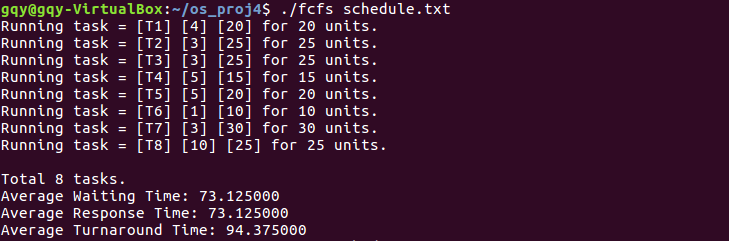
\includegraphics{fcfs}
		\caption{fcfs测试} \label{fcfs测试}
\end{figure}

测试指令如下
\begin{lstlisting}[language={[ANSI]C}]
make fcfs
./fcfs schedule.txt
\end{lstlisting}
首先用Makefile文件编译,生成fcfs可执行文件,输入./fcfs schedule.txt对schedule.txt的信息进行调度,测试结果如图 \ref{fcfs测试}。
\end{itemize}
%%%%%%%%%%%%%%%%%%%%%%%%%%%%%%%%%%%%%%%
\subsection{SJF}
\subsubsection{实验过程及步骤}
\begin{itemize}
\item[$\bullet$]创建全局变量,设计add函数,设计调度函数schedule()部分与FCFS类似,不作赘述
\item[$\bullet$]设计next\_tsk()函数运行下一个进程\\
由于是SJF调度,每次查找任务列表中运行时间最短的一个任务执行,然后将任务从任务列表中移除,并更新当前时间。寻找最短运行时间任务的时候需要遍历任务列表,用两个当前任务指针指向当前运行时间最短任务,另一个指针向后查找是否有更短运行时间的任务,如果有,就更新当前任务指针。另外需要为该进程计算相应的周转时间,等待时间,响应时间并更新全局变量记录信息。
\end{itemize}
\subsubsection{实验代码}
\begin{center}
{\ttfamily shedule\_sjf.c}
\end{center}
\begin{lstlisting}[language={[ANSI]C}]
# include <stdio.h>
# include <stdlib.h>
# include <string.h>

# include "task.h"
# include "list.h"
# include "cpu.h"
# include "schedulers.h"

struct node *head = NULL; 

//for calculating
int time = 0;		//current time.
int tsk_cnt = 0;	//task count.
int tt_wt_time = 0;	//total waiting time.
int tt_rsp_time = 0;	//total response time.
int tt_ta_time = 0;	//total turnaround time.
int tid_value = 0;	//task identifier
void add(char *name, int priority, int burst) {
	Task *tsk;
	tsk = (Task *) malloc (sizeof(Task));
	//avoid racing conditions
	tsk -> tid = __sync_fetch_and_add(&tid_value, 1);
	tsk -> name = (char *) malloc (sizeof(char) * (1 + strlen(name)));
	strcpy(tsk -> name, name);
	tsk -> priority = priority;
	tsk -> burst = burst;

	//for calculating
	tsk -> arv_time = time;	//arrival time.
	tsk -> wt_time = 0;	//waiting time.
	tsk -> last_exe_time = time;	//last execution time.
	tsk -> rsp_time = 0;	//response time.
	tsk -> ta_time = 0;	//turnaround time.
	insert(&head, tsk);	//add to list
}

void next_tsk() {
	if (head == NULL) return;
	
	struct node *cur = head;
	struct node *dex = head -> next;
	while (dex != NULL)	//sjf next
	{
		if(dex->task->burst <= cur->task->burst) cur = dex;
		dex = dex -> next;
	}
	Task *tsk = cur -> task;
	run(tsk, tsk -> burst);	//execute
	delete(&head, tsk);	//remove from list
	time += tsk -> burst;	//current time

	//for calculating
	//last waiting time.
	int last_wt_time = time - tsk -> last_exe_time - tsk -> burst;
	//waiting time.	
	tsk -> wt_time += last_wt_time;
	//response time.	
	if(tsk->last_exe_time==tsk->arv_time)//first exe
		tsk -> rsp_time = last_wt_time;
	//last execution time.	
	tsk -> last_exe_time = time;
	//turnaround time.
	tsk -> ta_time = time - tsk -> arv_time;
	
	//total data
	tsk_cnt += 1;
	tt_wt_time += tsk -> wt_time;
	tt_rsp_time += tsk -> rsp_time;
	tt_ta_time += tsk -> ta_time;

	//free
	free(tsk -> name);
	free(tsk);
}

void print() {
	printf("\nTotal %d tasks.\n", tsk_cnt);
	double avg_wt_time = 1.0 * tt_wt_time / tsk_cnt;
	double avg_rsp_time = 1.0 * tt_rsp_time / tsk_cnt;
	double avg_ta_time = 1.0 * tt_ta_time / tsk_cnt;
	printf("Average Waiting Time: %.6lf\n", avg_wt_time);
	printf("Average Response Time: %.6lf\n", avg_rsp_time);
	printf("Average Turnaround Time: %.6lf\n", avg_ta_time);
}

void schedule() {
	while (head != NULL)
		next_tsk();
	print();
}
\end{lstlisting}
\subsubsection{实验测试}
\begin{itemize}
\item[$\bullet$]sjf测试 (图 \ref{sjf测试})
\begin{figure}[htbp]
		\centering
		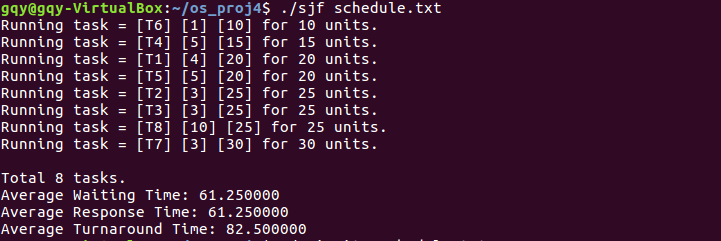
\includegraphics{sjf}
		\caption{sjf测试} \label{sjf测试}
\end{figure}

测试指令如下
\begin{lstlisting}[language={[ANSI]C}]
make sjf
./sjf schedule.txt
\end{lstlisting}
首先用Makefile文件编译,生成sjf可执行文件,输入./sjf schedule.txt对schedule.txt的信息进行调度,测试结果如图 \ref{sjf测试}。
\end{itemize}
%%%%%%%%%%%%%%%%%%%%%%%%%%%%%%%%%%%%%%%
\subsection{Priority scheduling}
\subsubsection{实验过程及步骤}
\begin{itemize}
\item[$\bullet$]创建全局变量,设计add函数,设计调度函数schedule()部分与FCFS类似,不作赘述
\item[$\bullet$]设计next\_tsk()函数运行下一个进程\\
由于是Priority scheduling调度,每次查找任务列表中优先级最高的一个任务执行,然后将任务从任务列表中移除,并更新当前时间。寻找最高优先级任务的时候需要遍历任务列表,用两个当前任务指针指向当前优先级最高任务,另一个指针向后查找是否有更高优先级的任务,如果有,就更新当前任务指针。另外需要为该进程计算相应的周转时间,等待时间,响应时间并更新全局变量记录信息。
\end{itemize}
\subsubsection{实验代码}
\begin{center}
{\ttfamily shedule\_priority.c}
\end{center}
\begin{lstlisting}[language={[ANSI]C}]
# include <stdio.h>
# include <stdlib.h>
# include <string.h>

# include "task.h"
# include "list.h"
# include "cpu.h"
# include "schedulers.h"

struct node *head = NULL; 

//for calculating
int time = 0;		//current time.
int tsk_cnt = 0;	//task count.
int tt_wt_time = 0;	//total waiting time.
int tt_rsp_time = 0;	//total response time.
int tt_ta_time = 0;	//total turnaround time.
int tid_value = 0;	//task identifier
void add(char *name, int priority, int burst) {
	Task *tsk;
	tsk = (Task *) malloc (sizeof(Task));
	//avoid racing conditions
	tsk -> tid = __sync_fetch_and_add(&tid_value, 1);
	tsk -> name = (char *) malloc (sizeof(char) * (1 + strlen(name)));
	strcpy(tsk -> name, name);
	tsk -> priority = priority;
	tsk -> burst = burst;

	//for calculating
	tsk -> arv_time = time;	//arrival time.
	tsk -> wt_time = 0;	//waiting time.
	tsk -> last_exe_time = time;	//last execution time.
	tsk -> rsp_time = 0;	//response time.
	tsk -> ta_time = 0;	//turnaround time.
	insert(&head, tsk);	//add to list
}

void next_tsk() {
	if (head == NULL) return;
	
	struct node *cur = head;
	struct node *dex = head -> next;
	while (dex != NULL)	//next priority highest
	{
		if(dex->task->priority >= cur->task->priority) cur = dex;
		dex = dex -> next;
	}
	Task *tsk = cur -> task;
	run(tsk, tsk -> burst);	//execute
	delete(&head, tsk);	//remove from list
	time += tsk -> burst;	//current time

	//for calculating
	//last waiting time.
	int last_wt_time = time - tsk -> last_exe_time - tsk -> burst;
	//waiting time.	
	tsk -> wt_time += last_wt_time;
	//response time.	
	if(tsk->last_exe_time==tsk->arv_time)//first exe
		tsk -> rsp_time = last_wt_time;
	//last execution time.	
	tsk -> last_exe_time = time;
	//turnaround time.
	tsk -> ta_time = time - tsk -> arv_time;
	
	//total data
	tsk_cnt += 1;
	tt_wt_time += tsk -> wt_time;
	tt_rsp_time += tsk -> rsp_time;
	tt_ta_time += tsk -> ta_time;

	//free
	free(tsk -> name);
	free(tsk);
}

void print() {
	printf("\nTotal %d tasks.\n", tsk_cnt);
	double avg_wt_time = 1.0 * tt_wt_time / tsk_cnt;
	double avg_rsp_time = 1.0 * tt_rsp_time / tsk_cnt;
	double avg_ta_time = 1.0 * tt_ta_time / tsk_cnt;
	printf("Average Waiting Time: %.6lf\n", avg_wt_time);
	printf("Average Response Time: %.6lf\n", avg_rsp_time);
	printf("Average Turnaround Time: %.6lf\n", avg_ta_time);
}

void schedule() {
	while (head != NULL)
		next_tsk();
	print();
}
\end{lstlisting}
\subsubsection{实验测试}
\begin{itemize}
\item[$\bullet$]priority测试 (图 \ref{priority测试})
\begin{figure}[htbp]
		\centering
		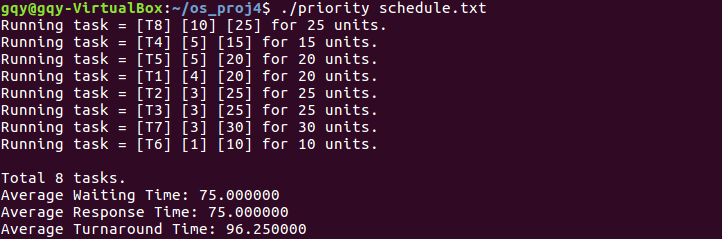
\includegraphics{p}
		\caption{priority测试} \label{priority测试}
\end{figure}

测试指令如下
\begin{lstlisting}[language={[ANSI]C}]
make priority
./priority schedule.txt
\end{lstlisting}
首先用Makefile文件编译,生成priority可执行文件,输入./priority schedule.txt对schedule.txt的信息进行调度,测试结果如图 \ref{priority测试}。
\end{itemize}
%%%%%%%%%%%%%%%%%%%%%%%%%%%%%%%%%%%%%%%
\subsection{RR}
\subsubsection{实验过程及步骤}
\begin{itemize}
\item[$\bullet$]创建全局变量,设计add函数,设计调度函数schedule()部分与FCFS类似,不作赘述
\item[$\bullet$]设计next\_tsk()函数运行下一个进程\\
由于是RR调度,每次执行任务列表中最先到达的任务,执行小于(剩余时间小于一个时间片)或等于一个时间片的时间,并更新当前时间。如果任务完成,就从任务列表删除该任务,并为它计算相应的周转时间,等待时间,响应时间并更新全局变量记录信息;否则将任务更新信息后插入回到到任务列表。根据任务列表插入方式,最先插入的进程在任务列表的最后,所以每次查找任务列表的最后一个并执行。
\end{itemize}
\subsubsection{实验代码}
\begin{center}
{\ttfamily shedule\_rr.c}
\end{center}
\begin{lstlisting}[language={[ANSI]C}]
# include <stdio.h>
# include <stdlib.h>
# include <string.h>

# include "task.h"
# include "list.h"
# include "cpu.h"
# include "schedulers.h"

struct node *head = NULL; 

//for calculating
int time = 0;		//current time.
int tsk_cnt = 0;	//task count.
int tt_wt_time = 0;	//total waiting time.
int tt_rsp_time = 0;	//total response time.
int tt_ta_time = 0;	//total turnaround time.
int tid_value = 0;	//task identifier
void add(char *name, int priority, int burst) {
	Task *tsk;
	tsk = (Task *) malloc (sizeof(Task));
	//avoid racing conditions
	tsk -> tid = __sync_fetch_and_add(&tid_value, 1);
	tsk -> name = (char *) malloc (sizeof(char) * (1 + strlen(name)));
	strcpy(tsk -> name, name);
	tsk -> priority = priority;
	tsk -> burst = burst;

	//for calculating
	tsk -> arv_time = time;	//arrival time.
	tsk -> wt_time = 0;	//waiting time.
	tsk -> last_exe_time = time;	//last execution time.
	tsk -> rsp_time = 0;	//response time.
	tsk -> ta_time = 0;	//turnaround time.
	insert(&head, tsk);	//add to list
}

void next_tsk() {
	if (head == NULL) return;
	
	struct node *cur = head;
	while (cur -> next != NULL) //next rr last one
		cur = cur -> next;
	Task *tsk = cur -> task;
	if(tsk -> burst <= QUANTUM)	//less than QUANTUM finish
	{	run(tsk, tsk -> burst);	//execute burst time
		delete(&head, tsk);	//remove from list
		time += tsk -> burst;	//current time

		//for calculating
		//last waiting time.
		int last_wt_time = time - tsk -> last_exe_time - tsk -> burst;
		//waiting time.	
		tsk -> wt_time += last_wt_time;
		//response time.	
		if(tsk->last_exe_time==tsk->arv_time)//first exe
			tsk -> rsp_time = last_wt_time;
		//last execution time.	
		tsk -> last_exe_time = time;
		//turnaround time.
		tsk -> ta_time = time - tsk -> arv_time;
	
		//total data
		tsk_cnt += 1;
		tt_wt_time += tsk -> wt_time;
		tt_rsp_time += tsk -> rsp_time;
		tt_ta_time += tsk -> ta_time;

		//free
		free(tsk -> name);
		free(tsk);
	}
	else	//more than QUANTUM
	{
		run(tsk, QUANTUM);	//execute QUANTUM
		delete(&head, tsk);
		time +=	QUANTUM;	//update current time
		//update task info for calculating
		tsk -> burst = tsk -> burst - QUANTUM;
		//last waiting time.
		int last_wt_time = time - tsk -> last_exe_time - QUANTUM;
		//waiting time.	
		tsk -> wt_time += last_wt_time;
		if(tsk->last_exe_time==tsk->arv_time)//first exe
			tsk -> rsp_time = last_wt_time;
		//last execution time.	
		tsk -> last_exe_time = time;
		
		insert(&head, tsk);	//add to list
	}
}

void print() {
	printf("\nTotal %d tasks.\n", tsk_cnt);
	double avg_wt_time = 1.0 * tt_wt_time / tsk_cnt;
	double avg_rsp_time = 1.0 * tt_rsp_time / tsk_cnt;
	double avg_ta_time = 1.0 * tt_ta_time / tsk_cnt;
	printf("Average Waiting Time: %.6lf\n", avg_wt_time);
	printf("Average Response Time: %.6lf\n", avg_rsp_time);
	printf("Average Turnaround Time: %.6lf\n", avg_ta_time);
}

void schedule() {
	while (head != NULL)
		next_tsk();
	print();
}
\end{lstlisting}
\subsubsection{实验测试}
\begin{itemize}
\item[$\bullet$]rr测试 (图 \ref{rr测试})
\begin{figure}[htbp]
		\centering
		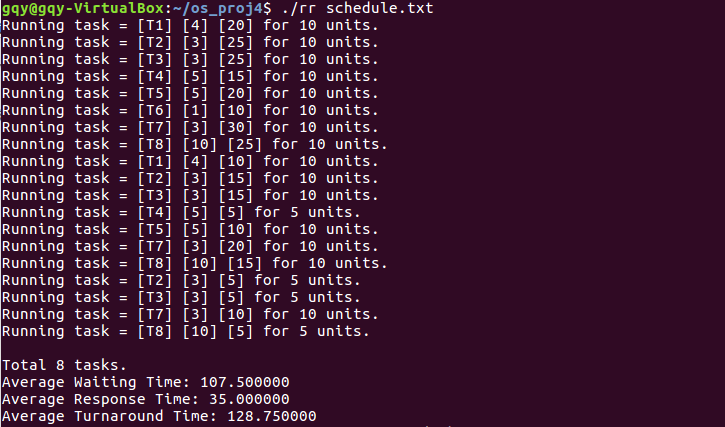
\includegraphics{rr}
		\caption{rr测试} \label{rr测试}
\end{figure}

测试指令如下
\begin{lstlisting}[language={[ANSI]C}]
make rr
./rr schedule.txt
\end{lstlisting}
首先用Makefile文件编译,生成rr可执行文件,输入./rr schedule.txt对schedule.txt的信息进行调度,测试结果如图 \ref{rr测试}。
\end{itemize}
%%%%%%%%%%%%%%%%%%%%%%%%%%%%%%%%%%%%%%%
\subsection{Priority with round-robin}
\subsubsection{实验过程及步骤}
\begin{itemize}
\item[$\bullet$]创建全局变量\\
由于Priority with round-robin调度需要根据优先级进行调度,所以全局变量的任务列表头结点设计为给每个优先级创建一个头结点,便于分优先级调度。
\item[$\bullet$]设计add函数部分\\
该函数其他部分与FCFS类似,只是插入任务的时候根据当前任务的优先级插入到相应优先级的头结点所在的列表中。
\item[$\bullet$]设计next\_tsk()函数运行下一个进程\\
由于是Priority with round-robin调度,这里设计的next\_tsk()函数有传入参数priority,表示选择该优先级下的任务列表的下一个任务执行。其他部分的实现跟RR调度类似,这里不作赘述。
\item[$\bullet$]设计调度函数schedule()\\
由于是Priority with round-robin调度,所以调度函数从最高优先级开始,根据优先级从高到低为每一个优先级队列调度,只有高优先级任务列表完成运行才会开始低优先级任务列表的调度。全部任务运行结束后打印计算结果。
\end{itemize}
\subsubsection{实验代码}
\begin{center}
{\ttfamily shedule\_priority\_rr.c}
\end{center}
\begin{lstlisting}[language={[ANSI]C}]
# include <stdio.h>
# include <stdlib.h>
# include <string.h>

# include "task.h"
# include "list.h"
# include "cpu.h"
# include "schedulers.h"

struct node *head[MAX_PRIORITY - MIN_PRIORITY + 1] = {}; 

//for calculating
int time = 0;		//current time.
int tsk_cnt = 0;	//task count.
int tt_wt_time = 0;	//total waiting time.
int tt_rsp_time = 0;	//total response time.
int tt_ta_time = 0;	//total turnaround time.
int tid_value = 0;	//task identifier
void add(char *name, int priority, int burst) {
	Task *tsk;
	tsk = (Task *) malloc (sizeof(Task));
	//avoid racing conditions
	tsk -> tid = __sync_fetch_and_add(&tid_value, 1);
	tsk -> name = (char *) malloc (sizeof(char) * (1 + strlen(name)));
	strcpy(tsk -> name, name);
	tsk -> priority = priority;
	tsk -> burst = burst;

	//for calculating
	tsk -> arv_time = time;	//arrival time.
	tsk -> wt_time = 0;	//waiting time.
	tsk -> last_exe_time = time;	//last execution time.
	tsk -> rsp_time = 0;	//response time.
	tsk -> ta_time = 0;	//turnaround time.
	insert(&head[priority- MIN_PRIORITY], tsk);	//add to list
}

void next_tsk(int priority) {
	if (head[priority- MIN_PRIORITY] == NULL) return;
	
	struct node *cur = head[priority- MIN_PRIORITY];
	while (cur -> next != NULL) //next priority_rr last one
		cur = cur -> next;
	Task *tsk = cur -> task;
	if(tsk -> burst <= QUANTUM)	//less than QUANTUM finish
	{	run(tsk, tsk -> burst);	//execute burst time
		delete(&head[priority- MIN_PRIORITY], tsk);	//remove from list
		time += tsk -> burst;	//current time

		//for calculating
		//last waiting time.
		int last_wt_time = time - tsk -> last_exe_time - tsk -> burst;
		//waiting time.	
		tsk -> wt_time += last_wt_time;
		//response time.	
		if(tsk->last_exe_time==tsk->arv_time)//first exe
			tsk -> rsp_time = last_wt_time;
		//last execution time.	
		tsk -> last_exe_time = time;
		//turnaround time.
		tsk -> ta_time = time - tsk -> arv_time;
	
		//total data
		tsk_cnt += 1;
		tt_wt_time += tsk -> wt_time;
		tt_rsp_time += tsk -> rsp_time;
		tt_ta_time += tsk -> ta_time;

		//free
		free(tsk -> name);
		free(tsk);
	}
	else	//more than QUANTUM
	{
		run(tsk, QUANTUM);	//execute QUANTUM
		delete(&head[priority- MIN_PRIORITY], tsk);
		time +=	QUANTUM;	//update current time
		//update task info for calculating
		tsk -> burst = tsk -> burst - QUANTUM;
		//last waiting time.
		int last_wt_time = time - tsk -> last_exe_time - QUANTUM;
		//waiting time.	
		tsk -> wt_time += last_wt_time;
		if(tsk->last_exe_time==tsk->arv_time)//first exe
			tsk -> rsp_time = last_wt_time;
		//last execution time.	
		tsk -> last_exe_time = time;
		
		insert(&head[priority- MIN_PRIORITY], tsk);	//add to list
	}
}

void print() {
	printf("\nTotal %d tasks.\n", tsk_cnt);
	double avg_wt_time = 1.0 * tt_wt_time / tsk_cnt;
	double avg_rsp_time = 1.0 * tt_rsp_time / tsk_cnt;
	double avg_ta_time = 1.0 * tt_ta_time / tsk_cnt;
	printf("Average Waiting Time: %.6lf\n", avg_wt_time);
	printf("Average Response Time: %.6lf\n", avg_rsp_time);
	printf("Average Turnaround Time: %.6lf\n", avg_ta_time);
}

void schedule() {
	for(int i = MAX_PRIORITY; i >= MIN_PRIORITY ; --i)
	{	
		while (head[i- MIN_PRIORITY]!= NULL)
		next_tsk(i);
	}
	print();
}
\end{lstlisting}
\subsubsection{实验测试}
\begin{itemize}
\item[$\bullet$]Priority with round-robin测试 (图 \ref{Priority with round-robin测试})
\begin{figure}[htbp]
		\centering
		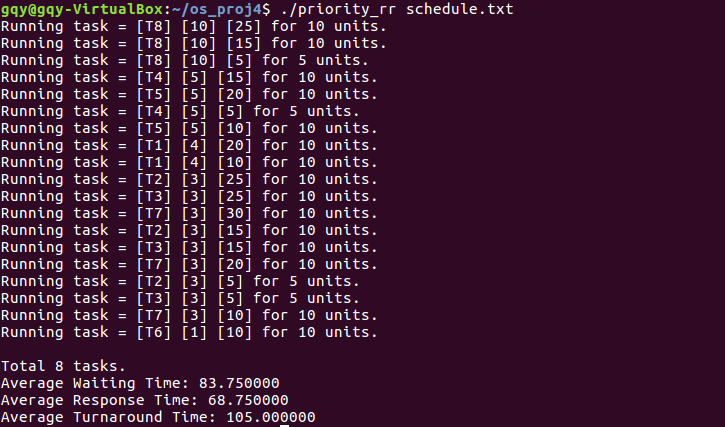
\includegraphics{prr}
		\caption{Priority with round-robin测试} \label{Priority with round-robin测试}
\end{figure}

测试指令如下
\begin{lstlisting}[language={[ANSI]C}]
make priority_rr
./priority_rr schedule.txt
\end{lstlisting}
首先用Makefile文件编译,生成priority\_rr可执行文件,输入./priority\_rr schedule.txt对schedule.txt的信息进行调度,测试结果如图 \ref{Priority with round-robin测试}。
\end{itemize}
%%%%%%%%%%%%%%%%%%%%%%%%%%%%%%%%%%%%%%%
\section{Conclusion}

\subsection{问题与解决方案}
本次project4分别实现了round-robin(RR), shortest-job-first(SJF), first-come,first-served(FCFS), priority scheduling, priority with round-robin五种进程调度算法,总体上难度不大,只要对所学知识有了解足够透彻就可以完成。其中priority with round-robin算法要结合优先级和RR算法调度,相较于别的算法实现起来比较困难,经过一番思考后决定采用分优先级的任务列表来实现,最终顺利完成了project。

\subsection{实验心得}
本次project4将五种进程调度算法实现出来,是对所学知识的一次很好地运用,算法实现难度并不大,但是需要仔细思考每一种算法的核心思想,采用合适的方法实现出来,比如在计算相应的时间信息的时候,需要在每次执行任务的时候及时维护更新时间信息,特别是RR算法以及priority with round-robin算法。总的来说本次project进一步加深了我对各类进程调度算法的理解,在算法实现的过程中也非常有成就感,让我受益匪浅。




%----------------------------------------------------------------------------------------


\end{document}